% 使用 xelatex 编译
\documentclass[UTF8,a4paper,twoside,zihao=-4,leqno]{ctexrep}
%%%% 文档类设置 %%%%%%%%
\ctexset{
	contentsname = {Contents},
	figurename = {Figure},
	tablename = {Table},
	bibname = {References},
	chapter = {
		beforeskip = 0pt,
		afterskip = 20pt,
		name = {Chapter\ },
		nameformat = \zihao{3}\bfseries,
		number = \Roman{chapter},
		numberformat = \zihao{3}\bfseries,
		titleformat = \zihao{3}\bfseries,
		fixskip = true,
		%afterindent = false
		        },
	section = {
		beforeskip = \ccwd,
		afterskip =1ex plus 0.2ex,
		format = \raggedright,
		nameformat = \zihao{4}\bfseries,
		numberformat = \zihao{4}\bfseries,
		titleformat = \zihao{4}\bfseries,
		%afterindent = false
			},
	subsection = {
		beforeskip =\ccwd,
		afterskip = 0.5ex,
		format = \raggedright,
		nameformat = \zihao{-4}\bfseries,
		numberformat = \zihao{-4}\bfseries,
		titleformat = \zihao{-4}\bfseries
			}
	    }

%%%% 宏包 %%%%%%%%%%%
\usepackage{amsmath,amssymb,amsfonts,mathrsfs}
\usepackage{graphicx}
\usepackage{ulem}
\usepackage{pdfpages}
\usepackage{lipsum}
\usepackage{booktabs}
\usepackage{array,tabularx,longtable}
	\newcolumntype{Y}{>{\centering\arraybackslash}X}
\usepackage{multirow,listings}
\usepackage{enumerate }
\usepackage{algorithm,algpseudocode}
\usepackage{tikz}
\usepackage{tikz-qtree,tikz-qtree-compat}
	\usetikzlibrary{arrows}
\usepackage[round]{natbib}
\usepackage{siunitx}
%%%%% 定理环境 %%%%%%%%%
\usepackage[thmmarks]{ntheorem}
{
  \theoremstyle{nonumberplain}
  \theoremheaderfont{\indent\bfseries}
  \theorembodyfont{\normalfont}
  \theoremsymbol{\ensuremath{\Box}}
  \newtheorem{proof}{Proof}
}
{
  \theoremheaderfont{\noindent\bfseries}
  \theorembodyfont{\normalfont}
  \newtheorem{theorem}{Theorem}[chapter]
  \newtheorem{lemma}{Lemma}[chapter]
  \newtheorem{definition}{Definition}[chapter]
  \newtheorem{axiom}{Axiom}[chapter]
  \newtheorem{corollary}{Corollary}[chapter]
}
%%%%%% 图表标题设置 %%%%%%%%%%%%%%%
\usepackage{caption}
%\DeclareCaptionLabelFormat{mylabel}{{\xeCJKsetup{CJKecglue={\hskip 0pt}}#1#2}}
\captionsetup{
		font= small,
		labelfont = bf,
		labelsep = space,
		%labelformat = mylabel
			}
\makeatletter
\renewcommand{\thefigure}{\ifnum \c@chapter>\z@ \thechapter-\fi \@arabic\c@figure}
\renewcommand{\thetable}{\ifnum \c@chapter>\z@ \thechapter-\fi \@arabic\c@table}
\makeatother

%%%% 页面设置 %%%%%%%%%%%%%%%%%%%%%%
\usepackage[bindingoffset=.5cm,centering,includeheadfoot,margin=2.5cm,headsep=1.5em]{geometry}
\setlength\parskip{0pt}
\usepackage{fancyhdr}\pagestyle{fancy}
\renewcommand\chaptermark[1]{%
	\markboth{\CTEXthechapter\quad #1}{}}
\renewcommand\sectionmark[1]{%
	\markright{\CTEXthesection\quad #1}}
\fancyhf{}
\fancyhead[LE,RO]{\thepage}
\fancyhead[RE]{\textsl{\nouppercase{\leftmark}}}
\fancyhead[LO]{\textsl{\nouppercase{\rightmark}}}
%\renewcommand{\headrulewidth}{0pt}

\usepackage[colorlinks,linkcolor=blue,citecolor=blue,bookmarks=true,bookmarksnumbered=true]{hyperref}
\usepackage{pdflscape}
%%%% 字体 %%%%%%%%%
\usepackage{lmodern}
\setCJKmainfont[
	BoldFont=AdobeHeitiStd-Regular.otf,
	ItalicFont=AdobeKaitiStd-Regular.otf
				]{simsun.ttc}
%%%%% 自定义命令 %%%%%%%%%%%%
\renewcommand{\bmod}{\ensuremath{\ \mathbf{mod}\ }}
\renewcommand{\div}{\ensuremath{\ \mathbf{div}\ }}
\newcommand{\remark}{\noindent\textit{\bfseries Remark:\ }}
\newcommand{\nequiv}{\not\equiv}
\renewcommand{\proof}{\noindent\textit{Proof:\ }}
\renewcommand{\qed}{\ensuremath{\hfill\Box}}
\renewcommand{\gets}{:=}
\newcommand{\TO}{\ensuremath{\ \textbf{to}\ }}
\newcommand{\return}{\textbf{return\ }}
\renewcommand{\leq}{\leqslant}
\renewcommand{\geq}{\geqslant}
\newcommand{\lcm}{\ensuremath{\text{lcm}}}
\newcommand{\algorithmautorefname}{Algorithm}
\newcommand{\lemmaautorefname}{Lemma}
\newcommand\sub[1]{\ensuremath{_{#1}}}
%%%%%%%%%%%%%%%%%%%%%%
%%%%%%%%%%%%%%%%%%%%%%
\begin{document}
\bibliographystyle{plainnat}
%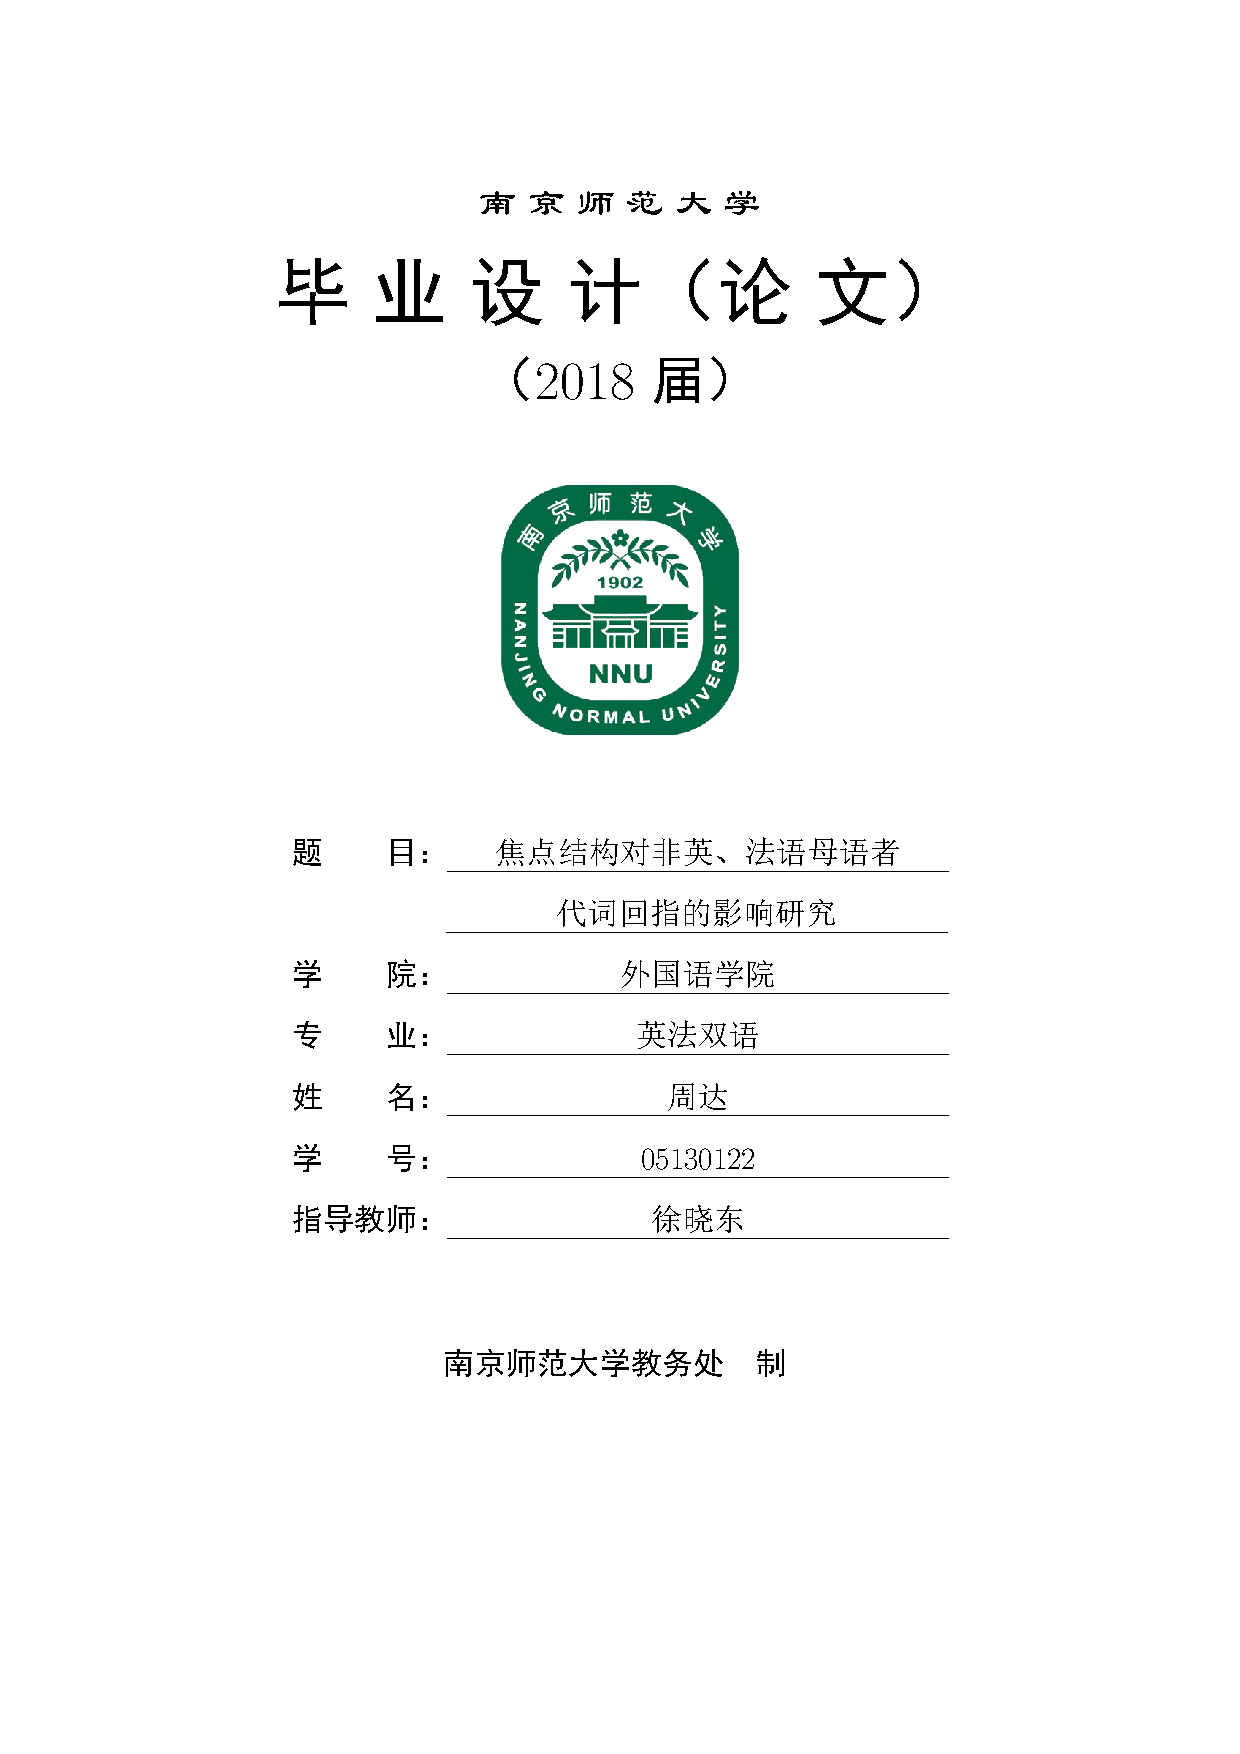
\includepdf{cover/cover.pdf} %%%%% 封面 %%%%%%%%%%%%
\newpage
\begin{titlepage}
\thispagestyle{empty}
\centering
\vspace*{3em}
\linespread{2}\selectfont
{\LARGE\bfseries 
The Impact of Focus Structure on Pronoun Resolution Among Non-native English and French Speakers}

\vspace{5em}
\linespread{1}\selectfont
\LARGE
Zhou Da

\bigskip
\Large
Under the Supervision of Xu Xiaodong

\vspace{5em}
\linespread{1.2}\selectfont
In Partial Fulfillment of \\
the Requirement for Bachelor's Degree\\
Submitted to\\
School of Foreign Languages and Cultures\\
Nanjing Normal University\\

\vspace{5em}
May, 2018

\end{titlepage}
%\newpage\mbox{}\thispagestyle{empty}\newpage
\newpage\mbox{}\thispagestyle{empty}\newpage
\pagenumbering{roman}
% acknowledgement

\clearpage
\thispagestyle{plain}
\phantomsection
\addcontentsline{toc}{chapter}{Acknowledgment}

\centerline{\zihao{3}\bfseries Acknowledgment}

\linespread{1.4}\zihao{-4}
\bigskip

I would like to thank my mentor Dr.\,Xu Xiaodong for his support and patience throughout the whole writing and editing process of this thesis. My gratefulness also goes to Liu Yunhan and Zhong Yuling who helped me to solve crucial problems in experiment design and implementation.

The thesis is typeset with \LaTeX. When preparing the format template, I got much help from numerous dedicated members of different \LaTeX\ communities, to whom I express my dearest thankfulness.
% Abstract
\clearpage
\thispagestyle{plain}
\phantomsection
\addcontentsline{toc}{chapter}{Abstract}

\centerline{\zihao{3}\bfseries Abstract}

\linespread{1.4}\zihao{-4}
\bigskip

This thesis explores the relationship between focus structure and pronoun resolution among non-native speakers of English and French. Firstly we reviewed the existing literature on the mechanism of focus effect and pronoun resolution. Then through a self-paced reading test, we find that focus, in the form of cleft structure does not necessarily increase the salience of a informational unit, thus may not in some cases make it a preferred antecedent for pronoun resolution. This result is line with previous researches on this topic. In our experiment, We also find that focused subject in French and focused object in English are processed faster, but focused subjects in both languages leads to longer response time of anaphora. Furthermore, our research also shows that the congruence between anaphora and focus does not make the latter more accessible. In this regard, we argue that the problem of whether there is subject or object preference in English and French is more complicated than the results of current studies.

\bigskip
\noindent\textbf{\zihao{4} Keywords:} 
focus effect, pronoun resolution, self-paced reading, English, French


%%% 中文摘要
\clearpage
\thispagestyle{plain}
\phantomsection
\addcontentsline{toc}{chapter}{摘\quad 要}

\centerline{\zihao{3}\heiti 摘\quad 要}

\linespread{1.4}\zihao{-4} \bigskip

本文探讨了英语和法语非母语者的语言处理过程中,焦点结构和代词回指之间的关系。首先我们从语法和语用角度,梳理了关于焦点作用和代词回指机制的研究现状。接着通过设计自定步速阅读实验,我们发现以分裂句为形式的焦点结构不一定能提升语言片段的显著性,并使其更可能成为代词回指的对象,这与前人的研究结果是相符的。在我们的测试中,法语主语位置的焦点和英语宾语位置的焦点反应时间都较短,但两种语言的主语焦点都导致了更长的回指反应时间。另外,我们还发现焦点和回指对象的一致性并不能提升焦点位置的显著性。因此本文认为,英语和法语中是否存在主语或宾语回指偏向的问题,比当前已有研究结论更加复杂。
\bigskip

\noindent{\zihao{4}\heiti 关键词:}
焦点作用, 代词回指, 自定步速阅读, 英语, 法语

\newpage\mbox{}\thispagestyle{empty}\newpage
\tableofcontents\thispagestyle{empty}
\newpage\mbox{}\thispagestyle{empty}\newpage
\clearpage\pagenumbering{arabic}

%%%%%%%%%% 正文 %%%%%%%%%%%%%%%%%%%%%%
%%%%%%%%%%%%%%%%%%%%%%%%%%%%%%%%%%%
%%%%%%%%%%%%%%%%%%%%%%%%%%%%%%%%%%%
%%%%%%%%%%%%%%%%%%%%%%%%%%%%%%%%%%%

\chapter{Introduction}
Anaphora, or referring backwards \citep{mitkov1999}, is a common linguistic tool for improving the efficiency of expressions. As in \eqref{mary}
\begin{align}
 \mbox{\emph{Mary dropped the cup. It shattered loudly.}} \label{mary}
\end{align}
the pronoun points to the cup clearly, thus exempting us from the labor of repetition at only a trivial distance. In daily usage of languages, we are constantly faced with the task of pronoun resolution. However, pronouns in some cases do not provide adequate information for identifying the intended referent. From time to time, we may also encounter ambiguous anaphora, whether be they literary devices or simply bad writings. Nevertheless, successful language production and comprehension requires rapid interpretation of co-references, which raises the questions of what factors determine our choices of antecedents for pronouns. The problem anaphora resolution has been an active area of research across many disciplines \citep{sayed2003}. However, resolving pronouns properly, whether for a human or a machine could be a difficult task since the referent could be at various syntax positions, and be distracted by semantic elements within or outside the same sentence. Furthermore, things can get more complicated when a discourse involves several parties or non-native speakers. 

In order to link the pronoun to its appropriate antecedent, people usually insert intentionally or subconsciously the referent into a salient position. The increase of the salience of a specific item in a sentence or discourse can be realized via various means, including topicalization, focus and focus-sensitive particles \citep{patterson2017}, which make up different information structures. \citet{徐晓东2014} distinguish linguistic (top-down) focus from non-linguistic (bottom-up) ones. The former includes cleft structure, which we will be focusing on in this thesis and wh-question etc.; and the latter mostly comprises of tonal changes, especially pitch accent. In practice, the syntactic aspect of focus is highly correlated with its phonological patterns. From the point of view of generative grammar, phonology and semantics cannot exchange information directly, so that syntactic mechanism including transformations, prosodic information, or focus in particular, is passed between semantics and phonology \citep{beaver2008}. Also unlike topicalization, which provides the theme of a sentence or discourse, namely what is being talked about, focus usually introduces “new, non-derivable, or contrastive information” \citep{halliday1967}, and is concerned about what is being said about. It should be noted that although the two notions serve different linguistic purposes, they are not contradictory to each other, so that focus might also be at topic position and vice versa.

Cleft is a primary implementation of focus in many languages. A cleft sentence is a complex sentence (the combination of a matrix clause and a dependent clause) that has a meaning that could be expressed by a simple sentence also known as the canonical sentence. Clefts typically put a particular constituent into focus. In spoken language, this focusing is often accompanied by a special intonation. In English, a cleft sentence can be constructed as follows:
\begin{align}
    \mbox{\emph{it}} + \mbox{\emph{conjugated form of to be}} + \left[X_F\right] + \mbox{\emph{subordinate clause}}
\end{align}
where \emph{it} is a cleft pronoun and $X$ is usually a noun phrase (although it can also be a prepositional phrase, and in some cases an adjectival or adverbial phrase). The focus is on X, or else on the subordinate clause or some element of it. For example, in \eqref{smith} and \eqref{joseph},
\begin{align}
    &\mbox{\emph{It's Mr. Smith (whom) we're looking for.}}\label{smith}\\
    &\mbox{\emph{It was from Joseph that she heard the news.}}\label{joseph}
\end{align}
\emph{Mr. Smith} and \emph{from Joseph} are focused. Furthermore, cleft structure usually induces an obligatory intonation break, so we may put a nuclear pitch accent on the focused constituents, which results in the interactions between phonology and semantics we mentioned earlier. Similarly, clefts can be achieved by \emph{c'est} (it is) structure in French:
\begin{align}
    &\mbox{\emph{C'est Jacque que je cherche.} (It's Jacque whom I'm looking for.)}\label{jacque}\\
    &\mbox{\emph{C'est à Paris que j'habite.} (It's in Paris where I live.)}\label{paris}
\end{align}
As can be seen from the examples above, focus can be either the subject or object of a sentence. If pronouns are introduced in later discourses, the focus can either be their antecedents or not. In addition, other factors such as topic, verb semantics, intra- and inter-sentential differences and even second language influence may come to play a role in the interpretation of pronouns. In this regard, the effectiveness of focus should be questioned in certain context.

The present study will thus explore the impact of focus effect on pronoun resolution of non-native English and French speakers, aiming to tackle three main problems:
\begin{itemize}
    \item how focus is formed syntactically in English and French;
    \item to what extent does focus increase the salience of the referent;
    \item and whether or not non-native English and French speakers respond to cleft structures in the same way as native speakers?
\end{itemize}
\chapter{Literature Review}

\section{Syntactic Approaches to Pronoun Resolution}
Syntactic structures play an important role in the interpretation of pronouns. \citet{ogrady2010} summarized several theories explaining the syntactic mechanism of pronoun resolution. First, they propose that reflexive pronoun and its antecedent must exist in the minimal inflection phrase (IP). Therefore in sentence like [\sub{\text{IP}}Claire knew that [\sub{\text{IP}}Alexis trusted her]] and [\sub{\text{IP}}Claire knew that [\sub{\text{IP}}Alexis trusted herself]], the pronoun \emph{her} points to to either Claire or the unmentioned third party, and the reflexive pronoun \emph{herself} can only mean Alexis.

Generative Grammar, especially the Government and Binding Theory also contributes to the clarification of rules behind pronoun resolution. One crucial model worth noticing is the c-command theory: 
\begin{definition}[C-Command]
	NP\sub{\text{a}} c-commands NP\sub{\text{b}} if the first category above NP\sub{\text{a}} contains NP\sub{\text{b}}.
\end{definition}
Stemming from the theory are two principles:
\begin{itemize}
	\item \textbf{Principle A}: A reflexive pronoun must have an antecedent that c-commands it in the same minimal IP;
	\item \textbf{Principle B}: A pronominal must not have an antecedent that c-commands it in the same minimal IP.
\end{itemize}
Therefore in \eqref{himself},
\begin{align}
	\mbox{\emph{That boy's teacher admires himself.}}\label{himself}
\end{align}
the reflexive pronoun himself can only be that boy's under Principle A, because as is illustrated in \autoref{fg:principlea}, \emph{that boy's teacher} c-commands \emph{himself}, the reflexive pronoun, in the same minimal IP.
\begin{figure}[htb]\centering
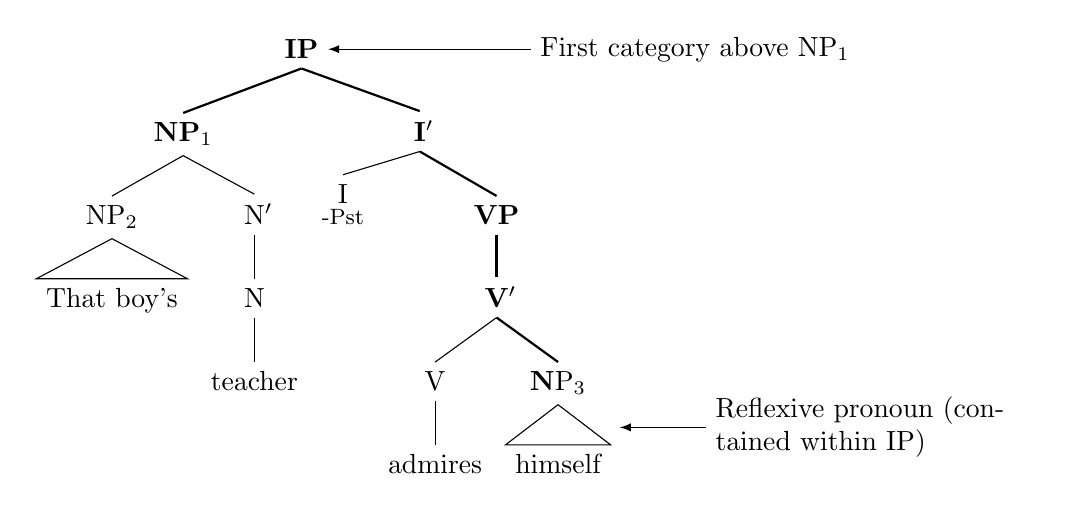
\begin{tikzpicture}[>=latex]
\tikzset{
	every tree node/.style={align=center,anchor=base}
}
\Tree [.\node(ip){\textbf{IP}}; \edge[thick]; 
				[.\textbf{NP\sub{1}} \qroof{That boy's}.NP\sub{2}
					   [.N\1 [.N teacher ] ] ]
		   \edge[thick]; [.\textbf{I\1} I\\[-1ex]{\footnotesize-Pst} 
		   \edge[thick]; [.\textbf{VP} 
		   		\edge[thick]; [.\textbf{V\1} [.V admires ] 
				   \edge[thick]; \node(rp){%
					   		\qroof{himself}.\textbf{NP\sub{3}}}; 
							   ] ] ] ]
\node(textip)[right of=ip,xshift=4cm]{First category above NP\sub{1}};
\node(textrp)[right of=rp,xshift=3cm,text width=4cm]
									{Reflexive pronoun 
									(contained within IP)};
\draw (ip) [<-] -- (textip); 
\draw (rp) [<-] -- (textrp);
\end{tikzpicture}
\caption{Structure illustrating c-command relations. NP\sub{1} c-commands NP\sub{3} but NP\sub{2} does not.}\label{fg:principlea}
\end{figure}

By contrast, in sentence like \eqref{him},
\begin{align}
	\mbox{\emph{That boy's teacher admires him.}}\label{him}
\end{align}
the pronoun him point solely to that boy, instead of anyone else, because under Principle B, \emph{that boy's teacher}, which c-commands the pronominal \emph{him} in the same minimal IP, should not its antecedent, as is clearly shown in \autoref{fg:principleb}.

\begin{figure}[htb]\centering
	\begin{tikzpicture}[>=latex]
		\tikzset{
			every tree node/.style={align=center,anchor=base}
		}
		\Tree [.\node(ip){IP}; \edge; 
						[.\node(np1){\textbf{NP\sub{1}}}; \qroof{That boy's}.\textbf{NP\sub{2}}
							   [.N\1 [.N teacher ] ] ]
				   \edge; [.I\1 I\\[-1ex]{\footnotesize-Pst} 
				   \edge; [.VP 
						   \edge; [.V\1 [.V admires ]\edge; \node(pr){\qroof{him}.NP\sub{3}}; 
									   ] ] ] ]
		\node(textip)[right of=ip,xshift=4cm]{First category above NP\sub{1}};
		\node(textpr)[right of=pr,xshift=3cm,text width=4cm]
											{Pronoun};
		\node(textnp1)[left of=np1,xshift=-3cm]{First category above NP\sub{2}};
		\draw (ip) [<-] -- (textip); 
		\draw (pr) [<-] -- (textpr);
		\draw (np1) [<-] -- (textnp1);
\end{tikzpicture}
\caption{Structure containing a pronominal}\label{fg:principleb}
\end{figure}

The explicitness of traditional syntactic approaches sometimes might seem too ideal for describing linguistic phenomena. As Sapir puts it, ``all grammar leaks'' \citep{manning1999}, it is impossible for us to characterize a complete and precise set of rules that seperate well-formed utterances from ill-formed ones, because we are constantly bending and evolving those ``rules'' in order to meet our changeable communicative needs. The rationalist approach towards language studies, especially the TG Grammar, has motivated major development in modern linguistics and computer science, but they are in the meantime inadequate, and sometimes na\"{i}ve, when in lack of more robust mathematical foundations \citep{kornai2008}. Therefore, along with the development of artificial intelligence, we are witnessing corpus-based statiscal methods being widely applied in more and more major linguistic fields to solve problems such as word-sense disambiguation and anaphora resolution.  

In more recent studies, for instance, dependency relations have also been taken into account in explaining the placing as well as the interpretation of anaphora. \citet{liu2017}, using data-driven analyses, find that there is a universal preference for dependency distance minimization (DDM), because the linear distance between two words related semantically or syntactically in one sentence, also are linked closely to our memory burden and syntactic complexity. Therefore, in the case of pronoun resolution, people tend to keep the referent at a closer position from the pronoun than other distracting words in the discourse, thus increasing the salience of the antecedent by reducing the syntactic zigzags.

\section{Exploring the Focus Effect}
Yet not everyone is familiar with the exact rules of anaphora or is equipped with a highly accurate probablistic analyzer, so that everyone is likely to generate ambiguous anaphora whether he or she is a native speaker or not. In writing guides such as \citet{pinker2014}, it is often advised that writers of all levels of proficiency should avoid ambiguous pronoun resolutions. Despite the challenges of understanding how human brain process anaphora, we are still able to perform complex pronoun resolutions every day without making errors. In practice, we quite intuitively pack key information into an easily accessible location for pronouns through both linguistic and non-linguistic approaches, among which focus is frequently used and is deemed as a gateway to the research of pronoun resolution.

Studies show different results on how focus affect pronoun resolution. \citet{徐晓东2013} argue that focus interact with other information structures i.e. topic, verb semantics and distance-related factors in the interpretation of pronouns. By using a writing completion test and two reading acceptability tests, they find that (1) antecedents are more likely to be referred to when topicalized than in the non-topic positions; and (2) forward biased verbs exert more influence on the determination of pronoun's referents than backward biased verbs do. Interestingly, \citet{徐晓东2013} in their study also propose that the modality of tasks adopted in experiments also has an influence over how topic structure and verb semantics affect pronoun resolution. That is, in sentence production test, topic has greater impact over anaphora than the implicit causal relations of verb semantics, but in sentence comprehension test, the direction of verb semantics seems to play a bigger role.

Some researches have also revealed L1 and L2 differences in pronoun resolution. \citet{patterson2017} conducted their experiment among native speakers of German and Russian, as well as non-native speakers of German whose mother tongue is Russian. Because Russian and German share similar patterns of focus construction, the impact of first language (Russian) on non-native language (German) pronoun resolution can be fairly excluded in the research. They discover that there is a clear difference of resolution preferences between native speakers and non-native speakers. For native speakers, they are less likely to resolve the pronoun to a clefted focus, which is termed as the “anti-focus effect”. However, non-native speakers do not show this tendency, and are often distracted by an antecedent accompanied by a focus-sensitive particle such as adverbs like “only” or “even”.

The argument that focus structure does not necessarily increase the salience of an antecedent is echoed by \citet{colonna2012}. They find that among native speakers of German and French, focusing reduces while topicalization enhances the accessibility of antecedents of pronouns within the same sentence. In a follow-up study, \citet{colonna2015} compare the focus effect in intra- and inter-sentential pronoun resolution in German. They point out that previous researches such as \citet{kaiser2011} and \citet{cowles2007} base their results on inter-sentence pronoun resolutions, namely conditions in which the pronoun and its antecedent are in different discourse units. While in \eqref{slap} 
\begin{align}
	\mbox{\emph{It is Peter who slapped John when he was young.}}\label{slap}
\end{align}
where the pronoun occur with its antecedent in the same sentence, the preference for the clefted focus was not observed. They further hypothesize that the so-called salience mechanisms, such as topicalization and cleft structure, should have a stronger effect between processing units (between sentences) than within a single processing unit where the semantics of the verb and the connective are assumed to play the most central role \citep{grosz1995}. 

In summary, focus is not an isolated factor of influence in pronoun resolution. Analysis of focus effect should be placed in the context of other information structures such as topic and perhaps verb semantic biases. The widely hold assumption that focus increases the sailience of a specific part of a discourse is no longer valid when intra- and inter-sentential differences are compared. Furthermore, the procedure of experiment should be considered, the format of which we believe is important, even decisive for subjects of experiments. Next, we will be reviewing the exsiting literature on a special type of focus, the cleft structure, and see its role in the anaphora resolution.

\section{Subject and Object Cleft Sentences}
The phenomenon that focus does not make the antecedent more accessible in intra-sentence experiments also finds explanation in the role of cleft in information structures. Almost all currently available studies agree that pronouns prefer topical antecedents. As a focused entity usually provides new and possibly unexpected information, it is not a good antecedent for a pronoun. However, the focus of an utterance may be related to the topic of the following one \citep{sgall1986}. More specifically, they propose that the cleft construction signals a potential topic-shift. Thus, a clefted antecedent may co-refer preferentially with a pronoun in a new sentence (or a new discourse unit) but not in the same sentence (or discourse unit). A topic-shift within a sentence (or discourse unit) reduces coherence whereas a topic-shift may occur in a new sentence (or a new discourse unit) without negatively affecting discourse coherence. 

Aside from the focus effect of cleft structure itself, several studies also have been working on the problem of whether there is a difference between subject and object cleft. \citet{kaiser2011}, for instance, investigated the focus effect of both focused subject and focused object in reference resolution. In order to put a contrastive focus on one of the potential antecedents (subject vs. object), she used discourse contexts in which one speaker corrected another speaker. It clefts (It was John that he congratulated vs. It was John who congratulated him) and SVO structures (He congratulated John vs. John congratulated him), both preceded by the same discourse context, were examined. Clefted, as compared to SVO structures, did not increase participant's off-line choices for a referent, regardless of whether the clefted referent was the subject or the object. However, the eye-movement data showed marginal effects of clefting as manifested in a late interaction ($1500\sim2000\,\si{ms}$ from pronoun onset), indicating increased fixations to focused subjects compared to other conditions.

\citet{reichle2014} also suggests such subject preference exists in anaphora resolution in French, despite object preference in English. He points out that while both English and French have versatile use of cleft structures, they are also affected by the different constraints on the formulation of focus. According to \citet{lambrecht2001}, a constraint allowing only topical material in preverbal subject position leads to an increased necessity to the use of clefts. Since preverbal subjects are generally topical, an agent receiving focal status is often expressed as an object (i.\,e.\,, in the focus phrase following the copula clause of the \emph{c'est} cleft) where it does not violate the language's prosodic and syntactic constraints. This use of the \emph{c'est} cleft, known as a subject cleft, marks focus on an NP referring to an agent that would have been a grammatical subject in the canonical version of the sentence. Conversely, an object cleft is a cleft that marks as focal an NP referring to a patient (the object in the canonical version of the sentence). 

In the light of these proposed constraints on French information structure and the language's reliance on clefts for focus marking, it has been claimed that the French \emph{c'est} cleft is ``more important'' than the English \emph{it} cleft, and that subjects are commonly marked as focal via \emph{c'est} clefts in French. Besides, \citet{reichle2014} also finds processing advantage of subject clefts over object clefts. The explanation is three-folds, including syntactic complexity, corpus-based distributional frequency of structures, and heuristic strategies depending on semantic or thematic information. \citet{engelkamp1982} also finds that readers prefer subjects in clefted position than objects, and that subjects are easier to comprehend, which is in line with previous researches that subject relative clause is also processed faster than object relative clause \citep{hakes1976}. They proceed claiming that in formulating a sentence, the speaker tends to adopt as grammatical subject that concept upon which his or her attention is focused. Therefore, in their view, both the subjectivisation of a referent and the clefting of new information are strategies that direct the reader or listener's attention to that part of the utterance. Thus, clefted subject has greater facilitative effect in anaphora resolution than clefted object.

However, in some cases where alternative non-ambiguous constructions exist, as is illustrated by \citet{colonna2012} in a cross-linguistic study of German and French, clefted object can also be preferred. Normally in French, when the subject of the matrix clause and that of the subordinate clause are co-referential, the use of the non-ambiguous infinitival structure is usually required, but co-reference with the object of the matrix clause can only be expressed with an explicit anaphora. Consequently, when presented with the sentence such as:
\begin{align}
	&\mbox{\emph{Le facteur a rencontré le balayeur avant qu'il rentre à la maison.}}\\
	\label{facteur}
	&\mbox{(\emph{The postal worker met the street-sweeper before he went home.})}\notag
\end{align}
French speakers can be influenced by the more idiomatic expression:
\begin{align}
	&\mbox{\emph{Le facteur a rencontré le balayeur avant de rentrer à la maison.}}\\
	\label{facteur2}
	&\mbox{(\emph{The postal worker met the street-sweeper before going home.})}\notag
\end{align}
Thus, the first redundant expression would force the reader or listener to pay extra attention to the inserted pronoun, and then resolve it to the object rather than the more natural subject.

So far in this section, we have delved deeper into the effect of subject-clefted focus and object-clefted focus discussed in several researches. We can conclude from the literature reviewed above that subject position seems to be more often used as focus, and clefted subject has better processing advantages than clefted object, although distractive factors come up in cases such as alternative non-ambiguous expressions. However, the argument that object preference in English \citep{reichle2014} is still questionable to us. In the following chapter, we will be verifying these results.
\chapter{The Current Study}

\section{Experiment Design}
In this study, we conducted a self-paced reading test in English and French respectively, aiming to explore how cleft structure affects pronoun resolution of non-native speakers of English and French. Both the test results of the selected sentences and the test procedure will be analyzed.

\subsection{Test Materials}
Twenty four groups of  non-ambiguous test sentences fall into six types (A--F) differed by their positions of focus and directions of anaphora, as are illustrated in \autoref{tb:corpus}. The selection of these test sentences adopts the method of \emph{Latin square}, thus each of the in total six lists contains twenty four sentences selected from each group, and each type of sentences occurs four times within each list. The benefit of this arrangement is that sentences in every list cover all six types, but do not come from the same group, so that subjects of the experiment picking one random list do not come cross sentences of the same semantic context. Because there are six lists, each list is tested three times.

The types of the sentences in every group are arranged as follows: \begin{enumerate}
    \item the pattern of anaphora is consistant, pointing to the subject and object of these sentences alternatively;
    \item type A and B are subject-clefted sentences; type C and D are object-clefted sentences;
    \item type E and F are sentences without focus structure.
\end{enumerate}   
Aside from twenty four test sentences selected from twenty four groups, each list also contains six \emph{filler items} (type G), which are sentences contains neither pronoun resolution nor cleft structure. All test sentences and filler items are of word length from seven to twelve, which is also a factor we take into consideration in our analysis. 

\subsection{Participants}
The participants are thirty-six final-year English and French major students from Nanjing Normal University. They all have beening learning English for over ten years, and are TEM-8 certificate holders. The French speaking participants have been learning the language for over three years, and they have TFS-4 certificates.

\subsection{Procedure}
The participants took full control of the pace of their reading by pressing the \textsf{SPACE} bottom to spontaneously display and hide consecutive words one by one of the test sentences. Response time for each word was recorded in miliseconds. We pay special attention to the response time of focus and anaphora positions of test sentences. Focus is the first word after \emph{It is} in English and \emph{C'est} in French. Anaphora takes the form of pronouns (he or she) in our tests.

In addition, half of the test sentences are followed by test questions, i.\,e.\,, either true or false statements relating to the previous sentences. Test questions, when displayed, participants press \textsf{A} on the keyboard if the statement is true based on the context and \textsf{L} if they do not match. For test sentences without following questions, participants simply press \textsf{SPACE} again to continue. Response time for test questions were also recorded.

\begin{landscape}\thispagestyle{empty}\centering
\begin{table}[htb]\caption{Test Materials}\label{tb:corpus}
\begin{tabular}{cp{.5\linewidth}p{.31\linewidth}c}
    \toprule
    \multicolumn{1}{l}{\textbf{Type}} & \multicolumn{1}{l}{\textbf{Test Sentence}} & \multicolumn{1}{l}{\textbf{Question}} & \multicolumn{1}{l}{\textbf{Answer}}\\
    \midrule
    A & It is Mary who hit Jason when she was in Paris. & \multirow{6}*{Mary was in New York.} & \multirow{6}*{\textsf{L}}\\
    B & It is Mary who hit Jason when he was in Paris. \\
    C & It is Jason whom Mary hit when she was in Paris. \\
    D & It is Jason whom Mary hit when he was in Paris. \\
    E & Mary hit Jason when she was in Paris. \\
    F & Mary hit Jason when he was in Paris. \\
    G & The bride invited the nun to her wedding & The nun was invited to the wedding. & \textsf{A} \\
    \midrule
    A & C'est Mary qui a frappée Jason quand elle était à Paris. & \multirow{6}*{Mary était à New York.} & \multirow{6}*{\textsf{L}} \\
    B & C'est Mary qui a frappée Jason quand il était à Paris.\\
    C & C'est Jason que Mary a frappé quand elle était à Paris.\\
    D & C'est Jason que Mary a frappe quand il était à Paris.\\
    E & Mary a frappée Jason quand elle était à Paris.\\
    F & Mary a frappée Jason quand il était à Paris.\\
    G & La Mariée a invitée la religieuse à son mariage. & La religieuse a été invitée à la mariage. & \textsf{A} \\
    \bottomrule
\end{tabular}
\end{table}
\end{landscape}


\section{Results}

We mesured the average response time for focus and anaphora positions as well as the questions, with the longest and the shortest response time filtered. In our experiment, participants take shorter time to process focus and longer time to process anaphora than words before and after the two positions in both languages. Detailed results are shown in \autoref{tb:rt_en} and \autoref{tb:rt_fr}. 

\begin{table}[htb]\caption{Average Response Time of English Test Materials}\label{tb:rt_en}
    \centering
    \begin{tabular}{lllllll}
        \toprule
        & A & B & C & D & E & F \\
        \midrule
        Focus & 283 & 253 & 223 & 260 \\
        Anaphora &  321 & 290 & 314 & 284 & 294 & 269 \\
        Question & 1734 & 1547 & 1143 & 1755 & 688 & 582 \\
        \bottomrule
    \end{tabular}
\end{table}

\begin{table}[htb]\caption{Average Response Time of French Test Materials}\label{tb:rt_fr}
    \centering
    \begin{tabular}{lllllll}
        \toprule
        & A & B & C & D & E & F \\
        \midrule
        Focus & 355 & 393 & 465 & 481 \\
        Anaphora & 446 & 351 & 333 & 539 & 349 & 447 \\
        Question & 3193 & 3349 & 2260 & 1910 & 656 & 549 \\
        \bottomrule
    \end{tabular}
\end{table}

Apart from focus and anaphora response time, we are also seeing that French verbs are processed longer than the English counterparts. Furthermore, we detected irregularly longer response time of some words sporadically.  For example, one participant spent \SI{1866}{ms} on the word \emph{whom} in the sentence \emph{It is Catherine whom Matthew arrested when she was living in Africa} (Type D, List A), while on focus and anaphora, the participant spent \SI{760}{ms} and \SI{447}{ms}, and around \SI{450}{ms} on other words. Another noticeable irregularity occurs in the sentence \emph{It is Michelle whom Roland mistreated when he was an adolescent}. One participant stayed for \SI{1183}{ms} on the word \emph{Roland}, and \SI{687}{ms} on \emph{adolescent}, but on other words, no more than \SI{346}{ms} was spent. 

\section{Discussion}
\subsection{General Analysis of English and French Data}
Generally, participants taking French tests tend to take longer time to read almost all testing units than participants taking English tests. The reason behind this result is two-fold: firstly, the participants have been learning English for over ten years, but they did not start taking French courses until entering college. Therefore, the profiency level of the L2 is a major cause of the difference between the response time of French and English; secondly, as we will be discussing later, French words are more complex morphologically, due to the conjugaison system. When encountering French verbs, participants also need to pay attention to the suffix \emph{-e}, if exists, which carries opposite meanings in subject and object-clefted sentences. For example, in 
\begin{align}
    \mbox{\emph{C'est Bella qui a hébergée Danis quand elle était célibataire.}}\\
    \label{bella}  
    \mbox{(\emph{It is Bella who housed Danis when she was single.})} \notag
\end{align}
the feminine form \emph{hébergée} signals that the agent, \emph{Bella}, is female, but in
\begin{align}
    \mbox{\emph{C'est Jane que Paul a aidée quand il vivait à Lyon.}}\\
    \mbox{(\emph{It is Jane whom Paul helped when he was in Lyon})} \notag
\end{align}
the word \emph{aidée} is suffixed by \emph{-e} only because the agent Jane is female.


However, there are some similar patterns in the two languages. In every list of French and English, focus processing appears to be more time-saving while anaphora resolution more time-consuming when compared with other testing units. We attribute this phenomenon to the memory burdens participants took during the tests. As the focused element usually occur at the beginning of a sentence (W3 in English and W2 in French), it becomes more prominent naturally and easier to be understood than anaphora which is usually located at the last four or five word. As other informational units drag memory burdens to the end of the sentence, it takes longer time for participants to recall the previous information, which is the same reason why response time for questions is even much longer. 

\subsection{Comparison with Previous Studies}
In our experiment, the result that focus does not necessarily render the antecedent more accesible in the same sentence is in line with \citet{colonna2015}. Data shows that non-focused sentence type E and F make the question--answer procedure significantly faster than that of sentence types with focus. Since focus and anaphora happen in the same test sentence, our results can be one proof of \citet{grosz1995}'s argument that focus is less prominent than other information structure within a single processing unit. From the point of view of syntactic complexity, we may also argue that the shorter sentence length of non-focused structure plays a bigger role here due to weaker challenges on short-time memory.

Subject preference in French and object preference in English, as proposed by \citet{reichle2014}, is verified in our tests, as indicated by the shorter processing time of focus of sentence type C and D in English and type A and B in French. Apart from the cognitive and grammatical evidence which suggests that the French \emph{c'est} structure enjoys special status \citep{lambrecht2001}, we may propose that the mandatory concatenation of \emph{cest} and \emph{est} in French, rather than optional form \emph{it's} in English helps the French focus to be put at a more forward and prominent position. However, in both languages, focused subject brought about longer response time of anaphora. The exact reason is is still a myth to us, and we either do not know why English objects are preferred, particularly by non-native speakers. 

Lastly, our experiment also finds that the congruence of focus and anaphora does not make the response of question easier. That is, the fact that anaphora points to focus does not improve the efficiency of pronoun resolution. In English materials, response time of anaphora in sentence type A and type C, where focus and anaphora are consistantly subject or object, is longer than that of sentence type B and type B where focus and anaphora do not match. In French materials, anaphora processing was sped up by object congruences, but was slowed by subject congruences. This discovery partly contradicts with the research of \citet{patterson2017}, according to whom, sentence type A and C should take less response time, which is however not the case in our study.

\subsection{Limitations}
One major factor of influence we have difficulty in assigning to the current logic is the exact cognitive approaches taken by the participants. We are not clear whether 
\begin{enumerate}
    \item certain words, or even names in our materials such as ``Santa Claus'' or ``Mary'' bear certain connotations or special memories for the participants so that they linger on this or even the next test sentence;
    \item they take distinct methodologies when offered the test materials of different languages;
    \item and their specific strategies have decisie influence on pronoun resolution.
\end{enumerate}
 Additionally, it needs to be clarified that to what extent does the response to the previous test sentences/questions affect the response time as well as the test-taking strategies of the following ones.

The different processing speeds among our participants can be both subtle and significant in the data collected. Indeed, some people are faster readers than others \citep{aravind2017}. However, a thorough explanation for the nuances in focus and anaphora processing requires the larger scale and more sophisticated corpus mining. Thus we cannot guarantee that our results will hold in other similar experiments. This problem of replicability \citep{brandt2014} also elicits us to doubt the effectiveness of the self-paced reading procedure, which is apparently not a perfect imitation of the normal reading process in the real world.  
\chapter{Conclusion}

Starting from the cleft sentences, we have explored the relationship between focus effect and pronoun resolution from a number of perspectives, including syntax, pragmatics and quantitative research data collected by others and our own experiment. We have seen that, focus as an special information structure is constantly interacting with other elements of discourses although it is usually assumed to have prominent cognitive status.

The results of our experiment agree with previous reseaches in some ways, such as the non-facilitative effect of focus in intra-sentential conditions, and the different preferences for antecedent in French and English pronoun resolution. However, some questions remain unsolved in our studies, including the precise mechanism behind object preference in English, the contradictory results about the congruence between focus and anaphora, and after all the influence of the specific reading strategies taken by the participants. The influence of L2 is explicitly reflected in the slower response time for nearly all test units in French, but whether L1 (Chinese) has an impact in our research still needs further verification. 

Focus marking and pronoun resolution are linguistic phenomena that involve complicated cognitive processes. In this regard, our experiment procedure is limited in many aspects. First of all is the scale. The number of test sentences as well as participants could be expanded. The second problem is the too simplistic experiment procedure and analytical methodology. We believe that the our research could be greatly improved by the inclusion of larger corpus materials and more mature statistical tools. Nevertheless, this thesis offers a glimpse into the studies of information structure and pronoun resolution. Hopefully, insights from our study could help further explorations in this field.




\begin{thebibliography}{99}
\addcontentsline{toc}{chapter}{References}

\bibitem[Aravind, Hackl \& Wexler(2017)]{aravind2017}
Aravind, A.\,, Hackl, M.\, \& Wexler, K.\,, 2017, Syntactic and Pragmatic Factors in Children's Comprehension of Cleft Constructions [J], \emph{Langauge Acquisition}, 1: 1-31.
\bibitem[Beaver \& Clark(2008)]{beaver2008}
	Beaver, D.\,I.\,\& Clark, B.\,Z.\,, 2008, \emph{Sense and Sensitivity: How Focus Determines Meaning} [M], Malden, MA: Blackwell Publishing.
\bibitem[Brandt et al(2014)]{brandt2014}
	Brandt, M.\,et al, 2014, The Replication Recipe: What makes for a convincing replication? [J], \emph{Journal of Experimental Social Psychology}, 50: 217--224.
\bibitem[Colonna, Schimke \& Hemforth(2012)]{colonna2012}
	Colonna, S.\,, Schimke, S.\,, \& Hemforth, B.\,, 2012, Information structure effects on anaphora resolution in German and French: A crosslinguistic study of pronoun resolution [J], \emph{Linguistics}, 55(5): 991--1013.
\bibitem[Colonna, Schimke \& Hemforth(2015)]{colonna2015}
	Colonna, S.\,, Schimke, S.\,, \& Hemforth, B.\,, 2015, Deifferent effects of focus in intra- and inter-sentential pronoun resolution in German [J], \emph{Language, Cognition and Neuroscience}, 30(10): 1306--1325.
\bibitem[Cowles, Walenski \& Kluender(2007)]{cowles2007}
	Cowles, H.\,H.\,, Walenski, M.\,, \& Kluender, R.\,, 2007, Linguistic and cognitive prominence in anaphora resolution: topic, contrastive focus and pronouns [J], \emph{Topoi}, 26(1): 3--18.
\bibitem[Grosz, Weinstein \& Joshi(1995)]{grosz1995}
	Grosz, B.\,J.\,, Weinstein, S.\,, \& Joshi, A.\,K.\,, 1995, Centering: A framework for modeling the local coherence of discourse [J], \emph{Computational Linguistics}, 21: 203--205.
\bibitem[Engelkamp \& Zimmer(1982)]{engelkamp1982}
	Engelkamp, J.\, \& Zimmer, H.\,D.\,, 1982, The interaction of subjectivization and concept placement in the processing of cleft sentences [J], \emph{Quarterly Journal of Experimental Psychology: Human Experimental Psychology}, 34(A): 463--478.
\bibitem[Hakes, Evans \& Brannon(1976)]{hakes1976}
	Hakes, D.\,T.\,, Evans, J.\,S.\, \& Brannon, L.\,L.\,, 1976, Understanding sentences with relative clauses [J], \emph{Memory and Cognition}, 4(3): 283--290.
\bibitem[Halliday(1967)]{halliday1967}
	Halliday, M.\,, 1967, Notes on Transitivity and Theme in English (Part 2) [J], \emph{Journal of Lingyuistics}, 3: 206.
\bibitem[Kaiser(2011)]{kaiser2011}
	Kaiser, E.\,, 2011, Focusing on pronouns: Consequences of subjecthooh, pronominalisation and contrastive focus [J], \emph{Language and cognitive Processes}, 26(10), 1625--1666.
\bibitem[Kornai(2008)]{kornai2008}
	Kornai, A.\,, 2008, \emph{Mathematical Linguistics} [M], London: Springer-Verlag. 
\bibitem[Lambrecht(2001)]{lambrecht2001}
	Lambrecht, K.\,, 2001, A framework for the analysis of cleft constructions [J], \emph{Linguistics}, 39(3): 463--516.
\bibitem[Liu, Xu \& Liang(2017)]{liu2017}
	Liu, H.\,, Xu, C.\, \& Liang, J.\,, 2017, Dependency distance: A new perspective on syntactic patterns in natural langauges [J], \emph{Physics of Life Reviews}, 21: 171--193.
\bibitem[Manning \& Sch\"{u}tze(1999)]{manning1999}
	Manning, C.\,D.\, \& Sch\"{u}tze, H.\,, 1999, \emph{Foundations of Statistical Natural Language Processing} [M], London: The MIT Press. 
\bibitem[Mitkov(1999)]{mitkov1999}
	Mitkov, R.\,, 1999, \emph{Anaphora Resolution: The State of the Art} [R], Paper based on the COLING'98/ACL'98 tutorial on anaphora resolution.
\bibitem[O'Grady et al(2010)]{ogrady2010}
	O'Grady, W.\, et al, 2010, \emph{Contemporary Linguistics: An Introduction} [M], Boston: Bedford \& St. Martin's.
\bibitem[Patterson, Esaulova \& Felser(2017)]{patterson2017}
	Patterson, C.\,, Esaulova, Y.\, \& Felser, C.\,, 2017, The impact of focus on pronoun resolution in native and non-native sentence comprehension [J], \emph{Second Langauge Research}, 33(4): 403--429.
\bibitem[Pinker(2014)]{pinker2014}
	Pinker, S.\,, 2014, \emph{The Sense of Style: The Thinking Person's Guide to Writing in the 21$^{st}$ Century} [M], New York: Penguin Books.
\bibitem[Reichle(2014)]{reichle2014}
	Reichle, R.\,, 2014, Cleft type and focus structure processing in French, \emph{Language, Cognition and Neuroscience}, 29(1): 107--124.
\bibitem[Sayed(2003)]{sayed2003}
	Sayed, I.\,Q.\,, 2003, \emph{Issues in Anaphora Resolution} [OL], retrieved from: \url{https://nlp.stanford.edu/courses/cs224n/2003/fp/iqsayed/project_report.pdf}.
\bibitem[Sgall, Hajicová \& Panevová(1986)]{sgall1986}
	Sgall, P.\,, Hajicová, E.\, \& Panevová, J.\,, 1986, \emph{The Meaning of the Sentence in its Semantic and Pragmatic Aspects} [M], Praha: Academia.
\bibitem[徐晓东, 陈庆荣(2014)]{徐晓东2014}
	徐晓东, 陈庆荣, 2014, 汉语焦点信息影响代词回指的电生理机制 [J], 《心理科学进展》, 22(6): 902--910.
\bibitem[徐晓东,倪传斌,陈丽娟(2013)]{徐晓东2013}
	徐晓东,倪传斌,陈丽娟, 2013, 话题结构和动词语义对代词回指的影响:一项基于语言产生和语言理解任务的实证研究 [J], 《现代外语(季刊)》, 36(4): 331--339. 
\end{thebibliography}

\end{document}